\documentclass[12pt,a4paper]{paper}
\usepackage[utf8]{inputenc}
\usepackage[english]{babel}
\usepackage{amsmath}
\usepackage{enumitem}
\usepackage{fixltx2e}
\usepackage{multicol}
\usepackage{amsmath}
\usepackage{enumitem}
\usepackage{arydshln}
\usepackage{amsfonts}
\usepackage{multirow}
\usepackage{multicol}
\usepackage{amssymb}
\usepackage{amsfonts}
\usepackage{amssymb}
\usepackage[left=1cm,right=1cm,top=1.5cm,bottom=2cm]{geometry}
\usepackage{Sweave}
\begin{document}
\title{STAT636 - Homework 5\\\small{Daniel Osorio - dcosorioh@tamu.edu\\Department of Veterinary Integrative Biosciences\\Texas A\&M University}}
\maketitle
\Sconcordance{concordance:HW5_DanielOsorio.tex:HW5_DanielOsorio.Rnw:%
1 17 1 1 0 9 1 1 2 1 0 1 4 3 0 3 1 3 0 1 2 3 1 1 7 6 0 1 1 6 0 2 2 1 0 %
1 3 2 0 1 1 6 0 1 2 3 1 1 2 1 0 3 1 4 0 1 2 1 1 1 2 1 0 1 8 11 0 1 2 3 %
1 1 2 1 0 1 1 1 3 2 0 1 1 6 0 1 2 1 8 7 0 1 1 6 0 1 2 1 4 3 0 1 1 6 0 2 %
2 7 0 1 2 7 0 3 1 4 0 1 2 13 1 1 2 1 0 5 1 1 3 2 0 2 1 3 0 2 2 4 0 1 2 %
3 1 1 2 1 0 2 1 8 0 1 2 6 0 1 2 6 0 1 2 7 0 2 2 1 0 2 1 8 0 1 2 6 0 1 2 %
6 0 1 2 7 0 1 2 1 1 1 2 1 0 1 4 3 0 1 3 2 0 1 6 8 0 1 2 1 1 1 2 1 0 1 2 %
1 0 1 2 1 0 1 1 4 0 1 2 1 3 7 0 3 1 1 2 9 0 1 2 6 0 1 2 6 0 1 2 7 0 1 2 %
3 1 1 2 1 0 3 1 3 0 1 2 1 1 1 2 1 0 1 1 11 0 1 2 1 1 1 2 1 0 1 1 8 0 1 %
2 6 0 1 2 6 0 1 2 7 0 1 2 3 1}

\begin{enumerate}
\item Consider the \texttt{Life\_Expectancy} data. Let the response $Y$ be \texttt{Life.expectancy}, and consider the numeric variables \texttt{Alcohol}, \texttt{percentage.expenditure}, \texttt{Total.expenditure}, \texttt{GDP}, \texttt{Income.composi-\\tion.of.resources}, and \texttt{Schooling} as the predictor variables; call these $x_1$, $x_2$, $\dots$, $x_6$, respectively. For the purpose of predicting the value of $Y$ , we will use linear regression models of the form
\begin{equation*}
y_{i} =\beta_{0} +\beta_{1}x_{1i} +\beta_{2}x_{2i} +\dots+\beta_{6}x_{6i} + \epsilon_{i}
\end{equation*}
Where $\epsilon_{i}$ are IID $\mathcal{N}(0,\,\sigma^{2})$, $i = 1, 2, \dots, n$
\begin{Schunk}
\begin{Sinput}
> lifeExpectancy <- read.csv("Life_Expectancy.csv")
> lifeExpectancy <- lifeExpectancy[,c(
+   "Life.expectancy", "Alcohol", "percentage.expenditure", 
+   "Total.expenditure", "GDP", "Income.composition.of.resources", 
+   "Schooling")]
> colnames(lifeExpectancy) <- c("Y", paste0("X",1:6))
> lifeExpectancy <- lifeExpectancy[complete.cases(lifeExpectancy),]
> N <- nrow(lifeExpectancy)
\end{Sinput}
\end{Schunk}
\begin{enumerate}
\item Using a usual least squares linear regression model (the \texttt{lm} function in R) (Using \texttt{na.omit} function to remove the row that there are some missing data.):
\begin{enumerate}
\item Use leave-one-out cross-validation to estimate the MSE of your model.
\begin{Schunk}
\begin{Sinput}
> SE <- sapply(seq_len(N), function(x){
+   model <- lm(formula = Y~., 
+               data = lifeExpectancy[-x,])
+   Yhat <- predict(model,lifeExpectancy[x,2:7, drop=FALSE])
+   return((lifeExpectancy[x,1] - Yhat)^2)
+ })
> mean(SE)
\end{Sinput}
\begin{Soutput}
[1] 26.58507
\end{Soutput}
\end{Schunk}
\item Use bootstrap (1000 times) to estimate the standard deviation of your MSE estimate. (\texttt{set.seed(2)} before sampling)
\begin{Schunk}
\begin{Sinput}
> set.seed(2)
> b <- sapply(seq_len(1000), function(x){
+   mean(sample(SE, replace = TRUE))
+ })
> sd(b)
\end{Sinput}
\begin{Soutput}
[1] 3.736676
\end{Soutput}
\end{Schunk}
\end{enumerate}
\item Make a diagnostics to check assumptions of the linear regression model in number 1. Specifically, please:
\begin{enumerate}
\item Make Normal QQ plot of residuals. Does the residuals appear normally distributed? \textit{Yes, residuals appears to be normally distributed}
\begin{Schunk}
\begin{Sinput}
> model <- lm(formula = Y~., data = lifeExpectancy)
> par(mar=c(3,3,2,1), mgp=c(2,0.5,0))
> qqnorm(residuals(model), pch = 20, las=1)
> qqline(residuals(model), col = "red")
\end{Sinput}
\end{Schunk}
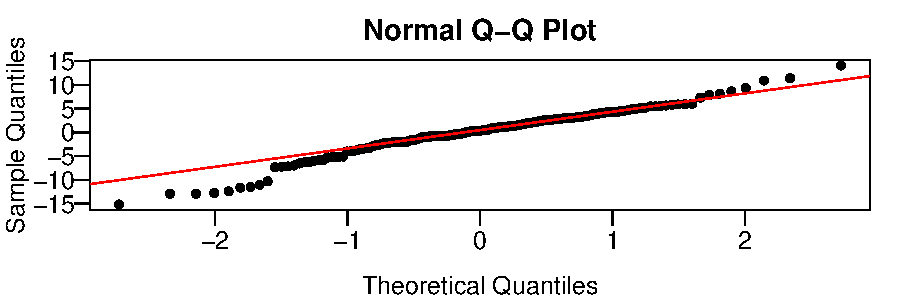
\includegraphics{HW5_DanielOsorio-004}
\item Create scatterplots for each covariate, with the covariate on x-axis and residuals on
y-axis. Do you see any problematic patterns? \textit{Yes, residuals are positively correlated with $x_{1}$, and variability is not equal across all the range in $x_{3}$ and $x_{5}$}
\begin{Schunk}
\begin{Sinput}
> par(mfrow=c(2,3),mar=c(3,3,2,1), mgp=c(2,0.5,0))
> scatterPlots <- sapply(1:6, function(x){
+   plot(y = residuals(model),
+        x = lifeExpectancy[,x], 
+        xlab = paste0("X",x), 
+        ylab = "Residuals", 
+        las =1, 
+        pch=20)
+ })
\end{Sinput}
\end{Schunk}
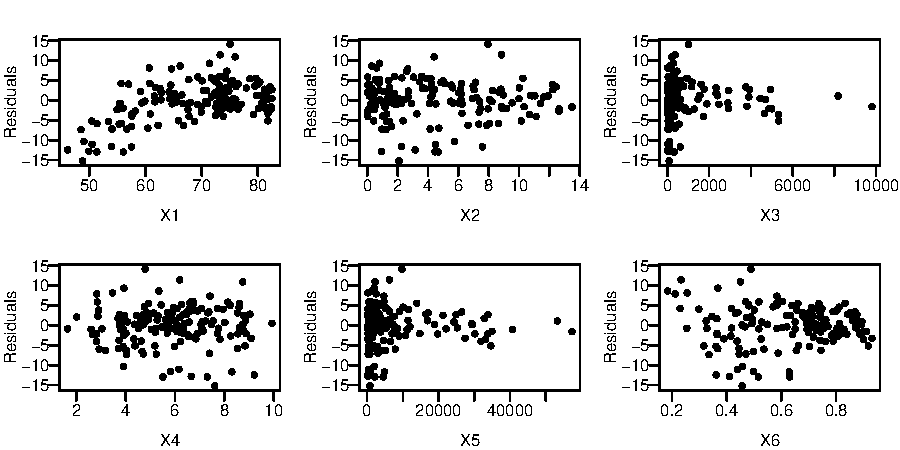
\includegraphics{HW5_DanielOsorio-005}
\end{enumerate}
\item Using regularized (lasso-based) linear regression (the \texttt{glmnet} and \texttt{cv.glmnet} functions from \texttt{glmnet} package in \texttt{R}, with \texttt{family=`gaussian'} and \texttt{alpha = 1}):
\begin{enumerate}
\item Based on cross-validation, using the \texttt{cv.glmnet} function, what is the optimal value of the tuning parameter \texttt{lambda}?
\begin{Schunk}
\begin{Sinput}
> X <- as.matrix(lifeExpectancy[,2:7])
> Y <- lifeExpectancy[,1]
> fittedModel <- glmnet::cv.glmnet(x = X, y = Y,
+                                  family = "gaussian", 
+                                  alpha = 1)
> print(lambda <- fittedModel$lambda.min)
\end{Sinput}
\begin{Soutput}
[1] 0.2007096
\end{Soutput}
\end{Schunk}
\item Use leave-one-out cross-validation (code it up yourself) and glmnet to estimate the MSE of the lasso model using the optimal tuning parameter.
\begin{Schunk}
\begin{Sinput}
> SE <- sapply(seq_len(N), function(z){
+   fittedModel <- glmnet::glmnet(x = X[-z,], y = Y[-z], 
+                                 family = "gaussian", 
+                                 alpha = 1, lambda = lambda)
+   Yhat <- predict(fittedModel,newx = X[z,,drop=FALSE])
+   return((Y[z] - Yhat) ^ 2)
+ })
> mean(SE)
\end{Sinput}
\begin{Soutput}
[1] 26.34441
\end{Soutput}
\end{Schunk}
\item Use bootstrap (again, code yourself, 1000 times) to estimate the standard deviation of your MSE estimate.
\begin{Schunk}
\begin{Sinput}
> b <- sapply(seq_len(1000), function(x){
+   mean(sample(SE, replace = TRUE))
+ })
> sd(b)
\end{Sinput}
\begin{Soutput}
[1] 3.536297
\end{Soutput}
\end{Schunk}
\item Compare the estimated $\beta$ coefficients from the lasso model (using $\lambda$ you gotten from (i)) to the least-squares model, and confirm that the lasso model’s coefficient estimates have been `shrunken' toward 0.
\begin{Schunk}
\begin{Sinput}
> as.numeric(coef(lm(formula = Y~.,data = lifeExpectancy)))
\end{Sinput}
\begin{Soutput}
[1]  4.057963e+01 -3.649839e-01  4.582845e-04  7.942828e-02  3.968866e-05
[6]  2.363990e+01  1.190499e+00
\end{Soutput}
\begin{Sinput}
> as.numeric(coef(glmnet::glmnet(x = X,y = Y,family = "gaussian",
+                                alpha = 1, lambda = lambda)))
\end{Sinput}
\begin{Soutput}
[1]  4.207565e+01 -1.869143e-01  2.382802e-04  0.000000e+00  4.923415e-05
[6]  2.312898e+01  1.074836e+00
\end{Soutput}
\begin{Sinput}
> fittedModel <- glmnet::glmnet(x = X,y = Y,family = "gaussian", alpha = 1)
> par(mar=c(3,3,2,1), mgp=c(2,0.5,0))
> plot(fittedModel, xvar = "lambda", label = TRUE, las=1)
\end{Sinput}
\end{Schunk}
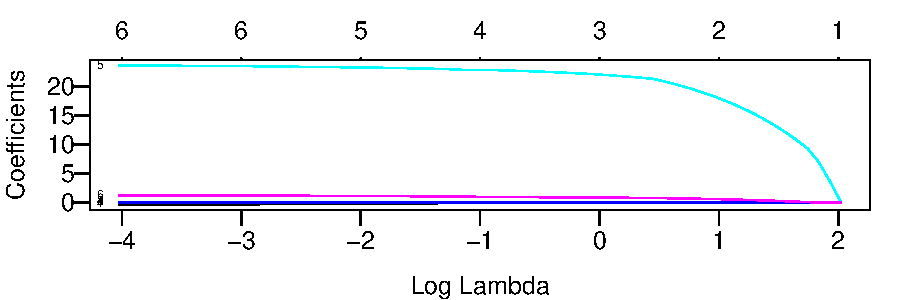
\includegraphics{HW5_DanielOsorio-009}
\end{enumerate}
\end{enumerate}
\item Consider the \texttt{HOF} data. Let the response $Y$ be the indicator for whether players are in the Hall of Fame (1 for “yes”, 0 for “no”), and consider the numerical variables \texttt{H}, \texttt{HR}, and \texttt{AVG} as the predictor variables (using \texttt{na.omit} before your job); call these $x_1$,$x_2$,$x_3$, respectively. Randomly split the $n = 1780$ training data sample observations into 2/3 for training and 1/3 for testing (Select 2/3 from data whose HOF is 1 and also 2/3 from data whose HOF is 0 and combine these two. Use \texttt{set.seed(2)} before sampling).\\ Let $p_i$ be the probability player $i$ is in the Hall of Fame, conditional on that player’s predictor variable values:
\begin{equation*}
p_i = Pr(Y_{i} = 1|x_{1i},x_{2i},x_{3i})
\end{equation*}
and consider the logistic regression model
\begin{equation*}
log\left(\frac{p_{i}}{1-p_{i}}\right) = \beta_0 +\beta_1x_{1i} +\beta_2x_{2i} +\beta{3}x_{3i}
\end{equation*}
for $i = 1, 2,\dots, n$. After fitting the model, obtaining parameter estimates $\hat{\beta}_{0}, \hat{\beta}_{1},\hat{\beta}_{2}$, we will predict Hall of Fame status for an individual with predictor variable values of $x^{*}_1$, $x^{*}_2$, $x^{*}_3$ based on his estimated probability $\hat{p}$, where
\begin{equation*}
\hat{p} = \frac{exp\left(\hat{\beta}_0 + \hat{\beta}_1x^{*}_1 + \hat{\beta}_2x^{*}_2 + \hat{\beta}_3x^{*}_3\right)}{1+exp\left(\hat{\beta}_0 + \hat{\beta}_1x^{*}_1 + \hat{\beta}_2x^{*}_2 + \hat{\beta}_3x^{*}_3\right)}
\end{equation*}
\begin{Schunk}
\begin{Sinput}
> set.seed(2)
> HOF <- read.csv("hof_data.csv")
> X <- HOF[,c("HOF","H", "HR", "AVG")]
> X[,1] <- as.numeric(X[,1])-1
> Y1 <- which(X[,1] == 1)
> Y0 <- which(X[,1] == 0)
> randomSelection <- c(
+   sample(x = Y1,size = round(length(Y1)*2/3)), 
+   sample(x = Y0,size = round(length(Y0)*2/3)))
> Training <- X[randomSelection,]
> Testing <- X[-randomSelection,]
\end{Sinput}
\end{Schunk}
Specifically, we will predict that $Y = 1$ if $\hat{p} > k$, for some choice of $k \in \left[0, 1\right]$. Fit the model to the training data:
\begin{Schunk}
\begin{Sinput}
> fittedModel <- glm(HOF~.,data=Training, family = "binomial")
\end{Sinput}
\end{Schunk}
\begin{enumerate}
\item Using the default choice of $k = 0.5$:
\begin{enumerate}
\item Report the misclassification rate, sensitivity, and specificity of your model when applied to the training data.
\begin{Schunk}
\begin{Sinput}
> hat <- predict(object = fittedModel, Training[,2:4], type = "response")
> hat <- ifelse(test = hat > 0.5,yes = 1, no = 0)
> print(ConfussionMatrix <- table(Observed=Training[,1],Predicted=hat))
\end{Sinput}
\begin{Soutput}
        Predicted
Observed   0   1
       0 638   7
       1  14  19
\end{Soutput}
\begin{Sinput}
> # Misclassification rate
> ConfussionMatrix[2,1]/sum(ConfussionMatrix[2,])
\end{Sinput}
\begin{Soutput}
[1] 0.4242424
\end{Soutput}
\begin{Sinput}
> # Sensitivity (True Positive Rate)
> ConfussionMatrix[2,2]/sum(ConfussionMatrix[2,])
\end{Sinput}
\begin{Soutput}
[1] 0.5757576
\end{Soutput}
\begin{Sinput}
> # Specificity (True Negative Rate)
> ConfussionMatrix[1,1]/sum(ConfussionMatrix[1,])
\end{Sinput}
\begin{Soutput}
[1] 0.9891473
\end{Soutput}
\end{Schunk}
\item Report the misclassification rate, sensitivity, and specificity of your model when applied to the test data. Comment of the relationship between the performance measures, testing compared to training. \textit{Missclassification rate (1-TPR): measures the proportion of positives which yield negative test outcomes with the test; Sensitivity (TPR): measures the proportion of actual positives that are correctly identified as such; Specificity (TNR): measures the proportion of actual negatives that are correctly identified as such.}
\begin{Schunk}
\begin{Sinput}
> hat <- predict(object = fittedModel, Testing[,2:4], type = "response")
> hat <- ifelse(test = hat > 0.5,yes = 1, no = 0)
> print(ConfussionMatrix <- table(Observed=Testing[,1],Predicted=hat))
\end{Sinput}
\begin{Soutput}
        Predicted
Observed   0   1
       0 319   3
       1   8   8
\end{Soutput}
\begin{Sinput}
> # Misclassification rate
> ConfussionMatrix[2,1]/sum(ConfussionMatrix[2,])
\end{Sinput}
\begin{Soutput}
[1] 0.5
\end{Soutput}
\begin{Sinput}
> # Sensitivity (True Positive Rate)
> ConfussionMatrix[2,2]/sum(ConfussionMatrix[2,])
\end{Sinput}
\begin{Soutput}
[1] 0.5
\end{Soutput}
\begin{Sinput}
> # Specificity (True Negative Rate)
> ConfussionMatrix[1,1]/sum(ConfussionMatrix[1,])
\end{Sinput}
\begin{Soutput}
[1] 0.9906832
\end{Soutput}
\end{Schunk}
\end{enumerate}
\item Now use leave-one-out (LOO) cross validation (CV) to `tune' the model with respect to $k$ on the training data, using misclassification rate as the guiding performance measure.
\begin{Schunk}
\begin{Sinput}
> N <- nrow(Training)
> LOO <- sapply(seq_len(N), function(x){
+   fittedModel <- glm(HOF~.,data=Training[-x,], family = "binomial")
+   predict(object = fittedModel, Training[x,2:4], type = "response")
+ })
> K <- sapply(seq(0,1,0.01), function(x){
+   as.numeric(LOO > x)
+ })
> ROC <- t(apply(K,2,function(hat){
+   ConfussionMatrix <- table(Observed=Training[,1],
+                             Predicted=factor(hat, levels = c(0,1)))
+   c(ConfussionMatrix[1,2]/sum(ConfussionMatrix[1,]),
+     ConfussionMatrix[2,2]/sum(ConfussionMatrix[2,]))
+ }))
\end{Sinput}
\end{Schunk}
\begin{enumerate}
\item Report an ROC curve.
\begin{Schunk}
\begin{Sinput}
> par(mar=c(4,4,1,1), mgp=c(1.6,0.5,0))
> plot(ROC, type = "l", ylab = "True Positive Rate", 
+      xlab = "False Positive Rate", main = "ROC", las = 1)
> optimalK <- which.max((order(ROC[,1],decreasing = FALSE) +
+                         order(ROC[,2], decreasing = FALSE))/2)
> abline(v=ROC[optimalK,1], col="red", lty = 2)
\end{Sinput}
\end{Schunk}
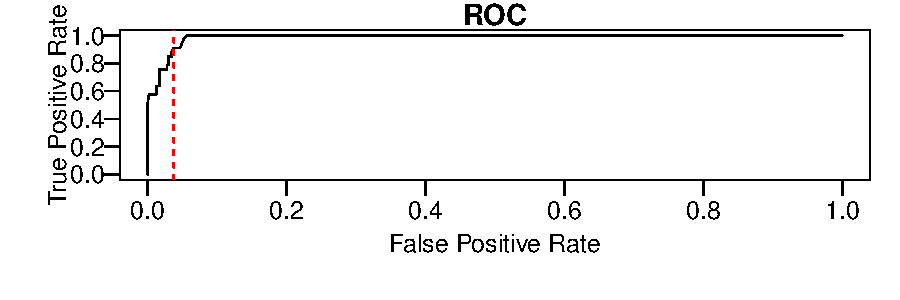
\includegraphics{HW5_DanielOsorio-015}
\item What is the optimal choice of $k$, and what are the CV-based estimates of misclassification rate, sensitivity, and specificity that correspond to this choice of $k$?
\begin{Schunk}
\begin{Sinput}
> # Optimal K
> seq(0,1,0.01)[optimalK]
\end{Sinput}
\begin{Soutput}
[1] 0.12
\end{Soutput}
\begin{Sinput}
> fittedModel <- glm(HOF~.,data=Training, family = "binomial")
> hat <- predict(object = fittedModel, Testing[,2:4], type = "response")
> hat <- ifelse(hat > seq(0,1,0.01)[optimalK], 1,0)
> print(ConfussionMatrix <- table(Observed=Training[,1],
+                                 Predicted=K[,optimalK]))
\end{Sinput}
\begin{Soutput}
        Predicted
Observed   0   1
       0 621  24
       1   3  30
\end{Soutput}
\begin{Sinput}
> # Misclassification rate
> ConfussionMatrix[2,1]/sum(ConfussionMatrix[2,])
\end{Sinput}
\begin{Soutput}
[1] 0.09090909
\end{Soutput}
\begin{Sinput}
> # Sensitivity (True Positive Rate)
> ConfussionMatrix[2,2]/sum(ConfussionMatrix[2,])
\end{Sinput}
\begin{Soutput}
[1] 0.9090909
\end{Soutput}
\begin{Sinput}
> # Specificity (True Negative Rate)
> ConfussionMatrix[1,1]/sum(ConfussionMatrix[1,])
\end{Sinput}
\begin{Soutput}
[1] 0.9627907
\end{Soutput}
\end{Schunk}
\end{enumerate}
\item Now we will perform the lasson on the training data.
\begin{enumerate}
\item Use cross-validation to choose the tuning parameter $\lambda$.
\begin{Schunk}
\begin{Sinput}
> X <- as.matrix(Training[,2:4])
> Y <- Training[,1]
> fittedModel <- glmnet::cv.glmnet(x = X, y = Y, family = "binomial")
> lambda <- fittedModel$lambda.min
\end{Sinput}
\end{Schunk}
\item Fit a lasso regression model on the training set and computing the coefficients using
$\lambda$ above.
\begin{Schunk}
\begin{Sinput}
> fittedModel <- glmnet::glmnet(X,Y,family = "binomial", lambda = lambda)
> coef(fittedModel)
\end{Sinput}
\begin{Soutput}
4 x 1 sparse Matrix of class "dgCMatrix"
                       s0
(Intercept) -13.144083522
H             0.004651503
HR            0.004065602
AVG           .          
\end{Soutput}
\end{Schunk}
\item Evaluate its misclassification rate, sensitivity and specificity on the training data
set using $\lambda$ which you get from above.
\begin{Schunk}
\begin{Sinput}
> hat <- round(predict(fittedModel, newx = X, type = "response"))
> print(ConfussionMatrix <- table(Observed=Training[,1], Predicted=hat))
\end{Sinput}
\begin{Soutput}
        Predicted
Observed   0   1
       0 639   6
       1  14  19
\end{Soutput}
\begin{Sinput}
> # Misclassification rate
> ConfussionMatrix[2,1]/sum(ConfussionMatrix[2,])
\end{Sinput}
\begin{Soutput}
[1] 0.4242424
\end{Soutput}
\begin{Sinput}
> # Sensitivity (True Positive Rate)
> ConfussionMatrix[2,2]/sum(ConfussionMatrix[2,])
\end{Sinput}
\begin{Soutput}
[1] 0.5757576
\end{Soutput}
\begin{Sinput}
> # Specificity (True Negative Rate)
> ConfussionMatrix[1,1]/sum(ConfussionMatrix[1,])
\end{Sinput}
\begin{Soutput}
[1] 0.9906977
\end{Soutput}
\end{Schunk}
\end{enumerate}
\end{enumerate}
\end{enumerate}
\end{document}
